\section{Experimental Evaluation}
\label{sec:experimental-evaluation}

In this section, we present the experimental results of \libname, comparing to Kernel Paxos 
%, an implementation of Multi-Paxos that reduces communication overhead by avoiding system calls and TCP/IP stack \cite{esposito2018kernel} 
and WbCast. % \cite{gotsman2019white}, another genuine atomic multicast protocol that takes as low as 3 message delays to deliver a message.
In Section~\ref{sec:evaluation:setup}, we describe the environment where we conducted our experiments and the parameters given to the different protocols.
In Section~\ref{sec:evaluation:micro}, we show the micro-benchmark results with different message sizes.
In Section~\ref{sec:evaluation:broadcast}, we exhibit the results for broadcast (i.e., multicast with a single group).
In Section~\ref{sec:evaluation:multicast}, we show throughput scales with the number of multicast groups for each protocol.


\subsection{Environment setup and configuration parameters}
\label{sec:evaluation:setup}

We conducted all experiments using the CloudLab infrastructure~\cite{DuplyakinATC19cloudlab} with two sets of nodes: 
(a) R320 node for broadcast experiments, equipped with one eight-core Xeon E5-2450 processor running at 2.1GHz, 16 GB of main memory, and a Mellanox FDR CX3 NIC; and (b) XL170 nodes for other experiments, equipped with one ten-core Intel E5-2640v4 processor running at 2.4GHz, 64 GB of main memory, and a Mellanox ConnectX-4 NIC. 
A 10 Gbps network link with around 0.1ms round-trip time connects all nodes running Ubuntu Linux 18.04 with kernel 4.15 an Oracle Java SE Runtime Environment 11. 

In all our experiments, there are client and server processes. 
Clients send requests in a closed-loop, i.e., each client multicasts a message to servers and waits for a response before multicasting the next message. 
In every protocol, each group has 3 processes with in-memory storage.

We defined three experimental setups:
in~\S\ref{sec:evaluation:micro} we deployed \libname with a single group and increasing message size;
\S\ref{sec:evaluation:broadcast} compares \libname with Kernel Paxos and WbCast in a broadcast (single-group) deployment;
\S\ref{sec:evaluation:multicast} presents a scenario with eight groups contrasting \libname and WbCast with an increasing number of clients and destination groups.

\subsection{Micro-benchmark: increasing message size}
\label{sec:evaluation:micro}
In this experiment, conducted on XL170 nodes, we measure \libname throughput and latency for different message sizes.
For each message size, from 64 bytes to 64 Kilobytes, we increase the number of clients until the system is saturated, i.e., throughput stops improving while latency raises.
Figure~\ref{fig:1group_message_size} (top) shows that messages up to 4KB long do not impact the overall system throughput, with nearly 250 thousand messages delivered each second. 
As the message size increases, the maximum throughput decreases with 35 thousand messages per second for 64KB messages.
The latency cumulative distribution function (CDF) in Figure~\ref{fig:1group_message_size} (bottom) exhibits minimum latency variation for messages with up to 4KB, around 20 microseconds.

\begin{figure}[htp!]
  \begin{subfigure}{\columnwidth}
    \centering
    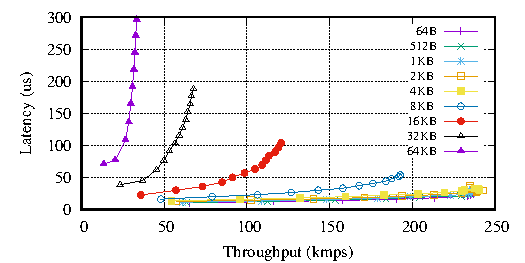
\includegraphics[width=0.99\columnwidth]{figures/benchmark/graphs/figure-performance-vs-size-single-group}
  \end{subfigure}
  \begin{subfigure}{\columnwidth}
    \centering
    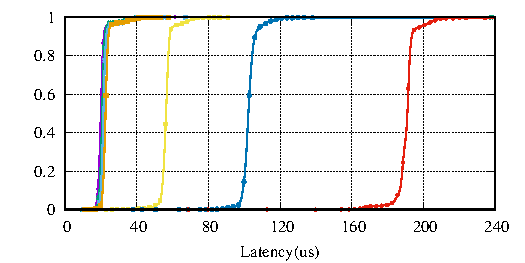
\includegraphics[width=0.95\columnwidth]{figures/benchmark/graphs/figure-performance-vs-size-single-group-cdf}
  \end{subfigure}
  \caption{\libname performance with different message sizes: throughput versus latency (top) and latency cumulative distribution function measured when the system is saturated (bottom)}
  \label{fig:1group_message_size}
\end{figure}

\subsection{Broadcast results}
\label{sec:evaluation:broadcast}

This experiment assesses how each protocol behaves in a scenario with a single group of three replicas for 64-byte and 1-kilobyte messages.
Figure~\ref{fig:broadcast} (top) shows that, for 64-byte messages, \libname outperforms the competitors with approximately 200 thousand messages per second. 
Kernel Paxos comes close with 170 thousand messages per second, while WbCast saturates sooner, with less than 60 thousand messages per second.
For larger messages, \libname kept the same performance, while the other protocols had the throughput reduced by half.
Figure~\ref{fig:broadcast} (bottom) confirms the superior results for \libname. The median latency for WbCast with small messages and a single client is nine times greater than the same measurement for our protocol.

\begin{figure}[htp!]
  \begin{subfigure}{\columnwidth}
    \centering
    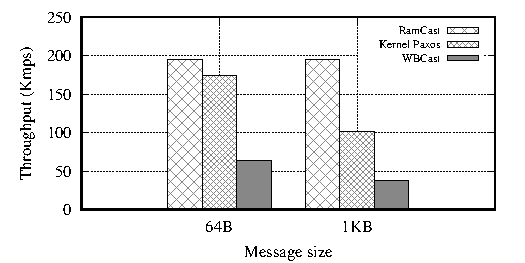
\includegraphics[width=0.99\columnwidth]{figures/benchmark/graphs/figure-compare-single-group-throughput}
  \end{subfigure}
  \begin{subfigure}{\columnwidth}
    \centering
    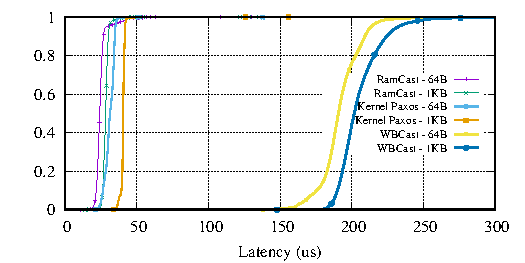
\includegraphics[width=0.95\columnwidth]{figures/benchmark/graphs/figure-compare-single-group-latency-cdf}
  \end{subfigure}
  \caption{Broadcast performance of \libname and competitors: throughput (top) and latency cumulative distribution function for a single client (bottom)}
  \label{fig:broadcast}
\end{figure}


\subsection{Multicast results: performance vs. number of destinations}
\label{sec:evaluation:multicast}

\begin{figure}[htp!]
  \begin{subfigure}{\columnwidth}
    \centering
    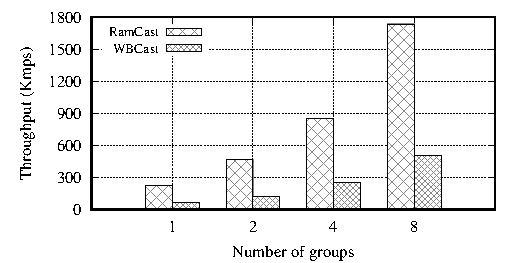
\includegraphics[width=0.99\columnwidth]{figures/benchmark/graphs/figure-genuine-compare-throughput}
  \end{subfigure}
  \begin{subfigure}{\columnwidth}
    \centering
    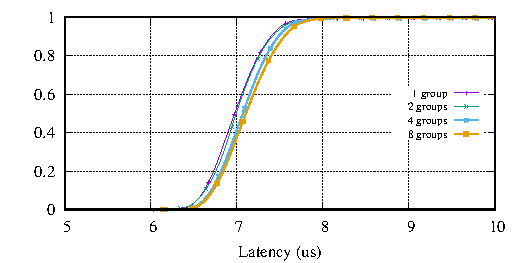
\includegraphics[width=0.95\columnwidth]{figures/benchmark/graphs/figure-genuine-compare-latency-cdf}
  \end{subfigure}
  \caption{Multicast performance of \libname and WbCast for single group messages: throughput (top) and latency cumulative distribution function of a \libname's (middle) and WbCast's single client (bottom)}
  \label{fig:tpcc_repartitioning2}
\end{figure}

\begin{figure}[htp!]
  \begin{subfigure}{\columnwidth}
    \centering
    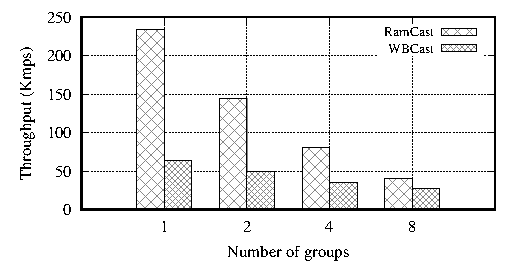
\includegraphics[width=0.99\columnwidth]{figures/benchmark/graphs/figure-multi-dest-compare-throughput}
  \label{fig:tpcc_repartitioning}
  \end{subfigure}
  \begin{subfigure}{\columnwidth}
    \centering
    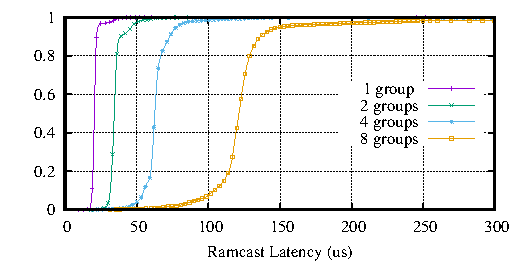
\includegraphics[width=0.95\columnwidth]{figures/benchmark/graphs/figure-multi-dest-compare-latency-cdf-ramcast}
  \end{subfigure}
  \begin{subfigure}{\columnwidth}
    \centering
    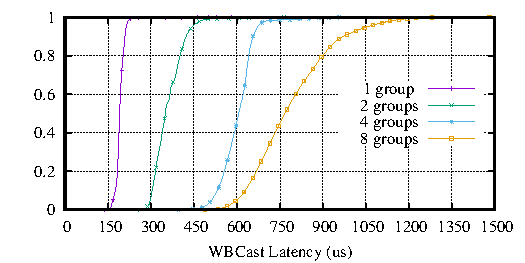
\includegraphics[width=0.95\columnwidth]{figures/benchmark/graphs/figure-multi-dest-compare-latency-cdf-wbcast}
  \end{subfigure}
  \caption{Performance comparison of \libname and WbCast for multi-groups message; throughput (top) and latency cumulative distribution function of \libname (middle) and WbCast (bottom)}
\end{figure}
